\section{Durchführung}
\label{sec:durchführung}

\subsection{Untersuchung eines Reflex-Klystrons}

Zunächst ist das Klystron in Betrieb zu nehmen und einzustellen.
Dazu wird das Klystron, wie in Abbildung~\ref{fig:aufbau1} dargestellt, an den Generator angeschlossen.
Es folgen der Isolator, ein Frequenzmesser und ein Dämpfungsmodul.
Zur Ermittlung der Frequenz des Klystrons wird am Generator die Reflektorspannung variiert und durch Erzeugen eines Minimums am SWR-Meter über den Frequenzmesser selbige gemessen.
Zur Untersuchung der verschiedenen Moden des Klystrons wird das SWR-Meter durch ein Oszilloskop ersetzt.
Durch Darstellen der Leistung gegen die Spannung können Modenkurven, wie in Abbildung~\ref{fig:moden} dargestellt, erzeugt werden.
Hierbei lässt sich die "Delle" auf der Spitze der Modenkurve mit dem Frequenzmesser verschieben. Die verschiedenen Flankeneinstellungen erfolgen über den Parameter der Reflektorspannung.
Es werden diese Spannungen, die Amplitude der Modenspitze und die Frequenz selbiger für alle Modenkurven aufgenommen.
%
\begin{figure}[h]
    \centering
    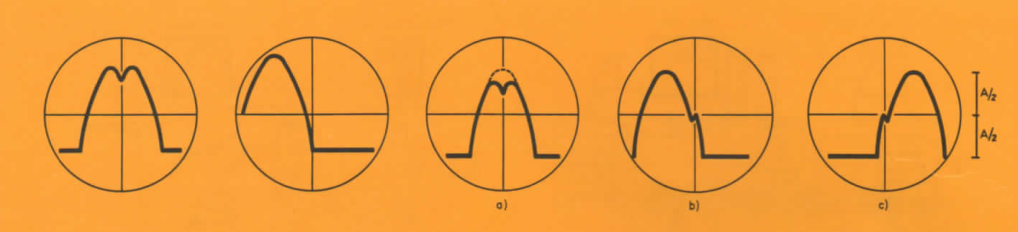
\includegraphics[width=0.85\textwidth]{figure/Moden.PNG}
    \caption{Darstellung der verschiedenen untersuchten Schwingungsmoden am Oszilloskop.\cite{V53}}
    \label{fig:moden}
\end{figure}
%
\begin{figure}[h]
    \centering
    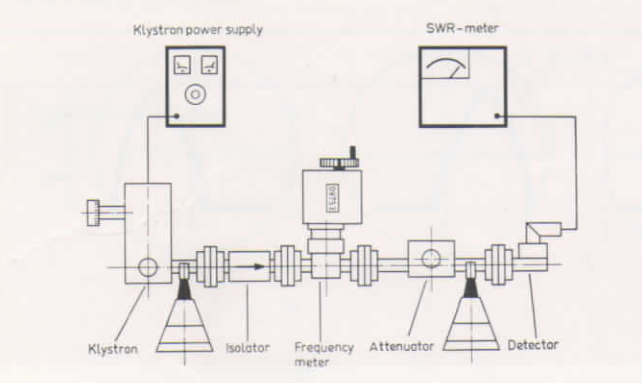
\includegraphics[width=0.8\textwidth]{figure/Aufbau_1.PNG}
    \caption{Aufbau des ersten Versuchsteils mit Klystron, Generator, SWR-Meter, Isolator, Frequenzmesser und Dämpfungsmodul.\cite{V53}}
    \label{fig:aufbau1}
\end{figure}

\subsection{Messung von Frequenz, Wellenlänge und Dämpfung}

Um die Klystronfrequenz aus der Wellenlänge zu bestimmen, wird die Amplitude von stehenden Wellen untersucht.
Dazu werden, wie in Abbildung~\ref{fig:aufbau2} dargestellt, ein Stehwellendetektor zur Untersuchung und ein Kurzschluss zur Erzeugung stehender Wellen in den Versuchsaufbau gebracht.
Zunächst wird hier die Frequenz über die oben beschriebene Methode mit Hilfe des Frequenzmessers in Verbindung mit dem SWR-Meter bestimmt.
Anschließend wird der Frequenzmesser wieder verstimmt.
Durch Verschieben des Stehwellendetektors kann über das SWR-Meter ein Minimum gefunden werden.
Der Abstand zweier solcher benachbarter Minima beträgt die halbe Wellenlänge der stehenden Welle.
Zur Bestimmung der Dämpfung wird der Kurzschluss durch einen Abschluss ersetzt.
Am Dämpfungsglied ist die Dämpfung sowie am SWR-Meter die Verstärkung \textsc{gain} so einzustellen, dass das SWR-Meter Vollauschlag anzeigt.
Über die Mikrometerschraube am Dämpfungsglied wird die Dämpfung (über eine Skala umrechenbar) variiert.
Die Leistungspegel am SWR-Meter werden aufgenommen und in $\SI{2}{\decibel}$ Schritten bis $\SI{10}{\decibel}$ erhöht.
Die gemessenen Dämpfungen werden durch die über die Skala aus der Schraubenposition Bestimmten ergänzt.

\begin{figure}[h]
    \centering
    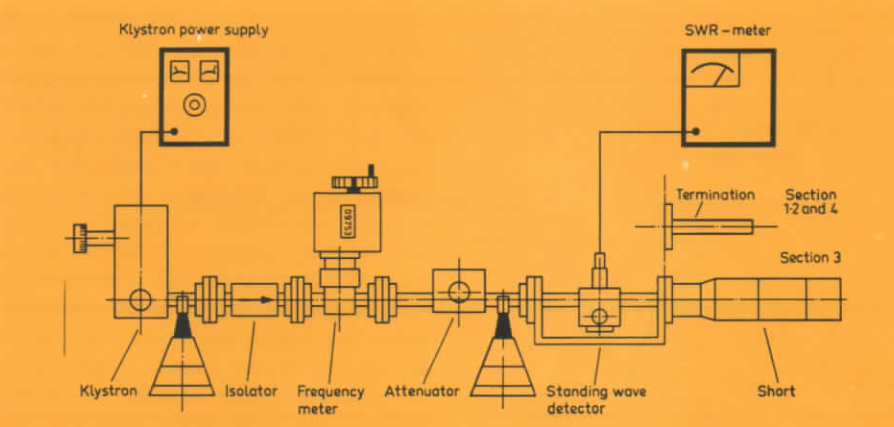
\includegraphics[width=0.8\textwidth]{figure/Aufbau_2.PNG}
    \caption{Aufbau des zweiten Versuchsteils mit Klystron, Generator, SWR-Meter, Isolator, Frequenzmesser und Stehwellendetektor.\cite{V53}}
    \label{fig:aufbau2}
\end{figure}

\subsection{Stehwellen-Messungen}

Im letzten Versuchsteil soll das Stehwellenverhältnis (SWR) bestimmt werden.
Dieses wird zunächst direkt über das SWR-Meter gemessen.
Dazu wird ein Gleitschraubentransformator vor den Kurzschluss gebaut~\ref{fig:aufbau3}.
Durch Variation der Position der Messsonde in ein Maximum kann über den \textsc{gain}-Regler das SWR zunächst auf 1 eingestellt werden.
Über das SWR-Meter lässt sich anschließend die Position eines Minimums für drei verschiedene Sondentiefen am Gleitschraubentransformator finden.
Hier wird das SWR abgelesen.
Über die $\SI{3}{\decibel}$-Methode wird ähnlich verfahren.
Die Messsonde wird bei fester Dämpfung in ein Minimum gebracht.
Dort wird der Verstärker am SWR so eingeregelt, dass sich ein Ausschlag von $\SI{3}{\decibel}$ einstellt.
Die Sonde wird nun nach links verschoben, bis sich ein Vollausschlag ergibt und ihre Position aufgenommen.
Dieses Vorgehen wird für eine Verschiebung nach rechts wiederholt.
Schließlich wird die Messung noch über die Abschwächer-Methode durchgeführt.
Dazu wird die Meßsonde bei fester Dämpfung ($\SI{20}{\decibel}$) in ein Minimum gebracht und die Verstärkung am SWR so eingestellt, dass sich ein Ausschlag von $\SI{3}{\decibel}$ ergibt.
Die Messsonde wird daraufhin entlang der Messleitung verschoben bis sich ein relatives Minimum ergibt.
An dieser Stelle wird die Dämpfung notiert, die nötig ist, um einen Ausschlag wie am Maximum zu erzeugen.

\begin{figure}[h]
    \centering
    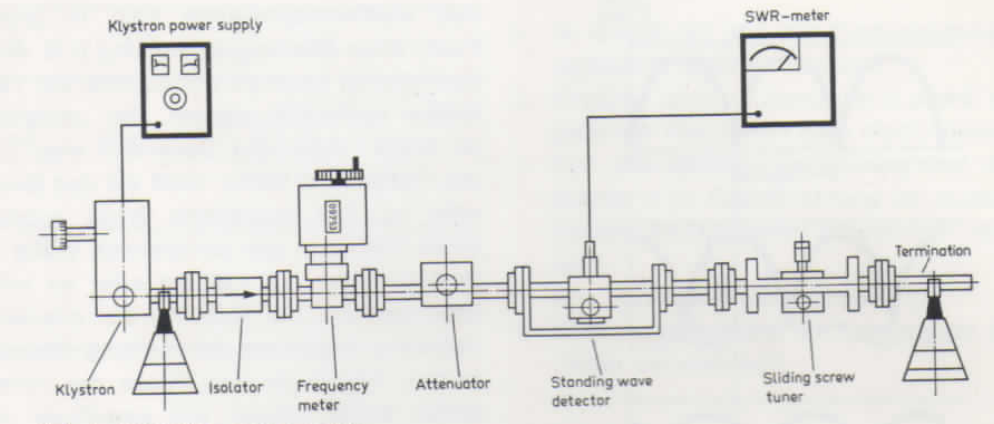
\includegraphics[width=0.8\textwidth]{figure/Aufbau_3.PNG}
    \caption{Aufbau des dritten Versuchsteils mit Klystron, Generator, SWR-Meter, Isolator, Frequenzmesser, Stehwellendetektor und Gleitschraubentransformator.\cite{V53}}
    \label{fig:aufbau3}
\end{figure}
